\runningheader{SAT Mathematics}{Drill Set 0}{Page \thepage\ of \numpages}

\begingradingrange{sat-drill-00}
\subsection*{SAT Drill 0}


\question[1]
\[
  C = \frac{5}{9}(F - 32)
\]
The equation above shows how temperature $F$, measured in degrees Fahrenheit, relates to a temperature $C$, measured in degrees Celsius. Based on the equation, which of the following must be true?

\statementbox{
  \begin{enumerate}[label=(\Roman*), itemsep=0.35em]
    \item A temperature increase of 1 degree Fahrenheit is equivalent to a temperature increase of $\frac{5}{9}$ degree Celsius.
    \item A temperature increase of 1 degree Celsius is equivalent to a temperature increase of $1.8$ degrees Fahrenheit.
    \item A temperature increase of $\frac{5}{9}$ degree Fahrenheit is equivalent to a temperature increase of 1 degree Celsius.
  \end{enumerate}
}

\begin{choices}
  \choice I only
  \choice II only
  \choice III only
  \CorrectChoice I and II only
\end{choices}

\question[1]
\[
  \frac{24x^2 + 25x - 47}{ax - 2} = -8x - 3 - \frac{53}{ax - 2}
\]
is true for all values of $x \neq \frac{2}{a}$, where $a$ is a constant. What is the value of $a$?

\begin{choices}
  \choice $-16$
  \CorrectChoice $-3$
  \choice $3$
  \choice $16$
\end{choices}


\newpage



\question[1]
If $3x - y = 12$, what is the value of $\displaystyle \frac{8^x}{2^y}$?

\begin{choices}
  \CorrectChoice $2^{12}$
  \choice $4^4$
  \choice $8^2$
  \choice The value cannot be determined from the information given.
\end{choices}

\question[1]
Points $A$ and $B$ lie on a circle with radius $1$, and arc $\stackrel{\frown}{AB}$ has length $\dfrac{\pi}{3}$. What fraction of the circumference of the circle is the length of arc $\stackrel{\frown}{AB}$?
\begin{solution}
$\dfrac{1}{6}$ \quad (\textit{equivalently} $0.166$ or $0.167$)
\end{solution}

\question[1]
The expression
\[
  \frac{8 - i}{3 - 2i}
\]
is rewritten in the form $a + bi$, where $a$ and $b$ are real numbers. What is the value of $a$? (Note: $i = \sqrt{-1}$.)
\begin{solution}
$2$
\end{solution}



\newpage



\question[1]
In triangle $ABC$, the measure of $\angle B$ is $90^\circ$, $BC = 16$, and $AC = 20$. 
Triangle $DEF$ is similar to triangle $ABC$, with vertices $D$, $E$, and $F$ corresponding 
to $A$, $B$, and $C$ respectively, and each side of triangle $DEF$ is $\dfrac{1}{3}$ the 
length of the corresponding side of triangle $ABC$. What is the value of $\sin F$?
\begin{solution}
$\dfrac{3}{5}$ \quad (\textit{equivalently} $0.6$)
\end{solution}


\question[1]
The incomplete table below summarizes the number of left-handed and right-handed students by gender for the eighth grade students at Keisel Middle School.
\begin{center}
  \renewcommand{\arraystretch}{1.3}
  \setlength{\tabcolsep}{0.6em}
  \begin{tabular}{|l|c|c|}
    \hline
    & \textbf{Left-handed} & \textbf{Right-handed} \\ \hline
    \textbf{Male}   & \hspace{1.2cm} & \hspace{1.2cm} \\ \hline
    \textbf{Female} & \hspace{1.2cm} & \hspace{1.2cm} \\ \hline
    \textbf{Total} & 18 & 122 \\ \hline
  \end{tabular}
\end{center}
There are 5 times as many right-handed female students as left-handed female students, and 9 times as many right-handed male students as left-handed male students. If there are 18 left-handed students and 122 right-handed students in total, which of the following is closest to the probability that a right-handed student selected at random is female? (Assume that no eighth-grade student is both right-handed and left-handed.)

\begin{choices}
  \CorrectChoice $0.410$
  \choice $0.357$
  \choice $0.333$
  \choice $0.250$
\end{choices}



\newpage



\uplevel{%
  \textbf{For questions 8 and 9, use the following information.}\par\smallskip
  If shoppers enter a store at an average rate of $r$ shoppers per minute and each stays an average of $T$ minutes, the average number of shoppers in the store, $N$, at any one time is given by
  \[
    N = rT
  \]
  (Little's law). The owner of the Good Deals Store estimates that during business hours, an average of 3 shoppers per minute enter the store and each stays an average of 15 minutes, so there are about 45 shoppers in the store at any time.%
}

\question[1]
Little's law can be applied to any part of the store. The store owner determines that during business hours, approximately 84 shoppers per hour make a purchase and each spends an average of 5 minutes in the checkout line. At any time during business hours, about how many shoppers, on average, are waiting in the checkout line to make a purchase at the Good Deals Store?
\begin{solution}
$7$
\end{solution}

\question[1]
The owner opens a new store across town. For the new store, an average of 90 shoppers per hour enter and each stays an average of 12 minutes. The average number of shoppers in the new store at any time is what percent less than the average number in the original store? (Ignore the percent symbol when entering your answer; e.g., if the answer is $42.1\%$, enter $42.1$.)
\begin{solution}
$60$
\end{solution}



\newpage



\question[1]
In the $xy$-plane, the point $(p, r)$ lies on the line $y = x + b$, and the point $(2p, 5r)$ lies on the line $y = 2x + b$, where $b$ is a constant. If $p \neq 0$, what is the value of $\dfrac{r}{p}$?

\begin{choices}
  \choice $\frac{2}{5}$
  \CorrectChoice $\frac{3}{4}$
  \choice $\frac{4}{3}$
\end{choices} 

\question[1]
A grain silo is built from two right circular cones and a right circular cylinder with internal measurements represented by the figure below. Of the following, which is closest to the volume of the grain silo, in cubic feet?
\begin{center}
  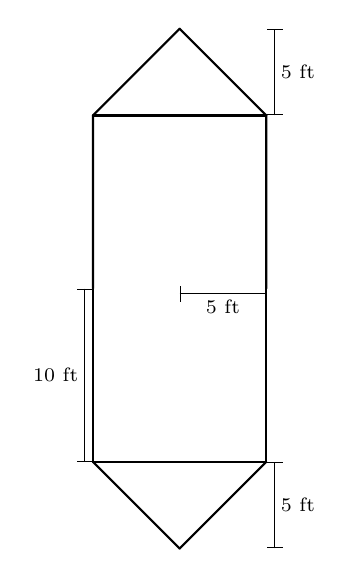
\begin{tikzpicture}[x=0.22cm, y=0.22cm, line cap=round, line join=round]
    \def\r{5}
    \def\Hcyl{10}
    \def\Hcone{5}
    \draw[thick] (0,\Hcyl+\Hcone) -- (-\r,\Hcyl) -- (-\r,0);
    \draw[thick] (0,\Hcyl+\Hcone) -- (\r,\Hcyl) -- (\r,0);
    \draw[thick] (-\r,\Hcyl) -- (\r,\Hcyl);
    \draw[thick] (-\r,0) -- (-\r,-\Hcyl);
    \draw[thick] (\r,0) -- (\r,-\Hcyl);
    \draw[thick] (-\r,-\Hcyl) -- (\r,-\Hcyl);
    \draw[thick] (-\r,-\Hcyl) -- (0,-\Hcyl-\Hcone);
    \draw[thick] (\r,-\Hcyl) -- (0,-\Hcyl-\Hcone);
    \draw[|-|] (-\r-0.5,0) -- (-\r-0.5,-\Hcyl) node[midway,left,inner sep=2pt] {\scriptsize 10 ft};
    \draw[|-|] (0,-0.3) -- (\r,-0.3) node[midway,below,inner sep=2pt] {\scriptsize 5 ft};
    \draw[|-|] (\r+0.5,\Hcyl) -- (\r+0.5,\Hcyl+\Hcone) node[midway,right,inner sep=2pt] {\scriptsize 5 ft};
    \draw[|-|] (\r+0.5,-\Hcyl-\Hcone) -- (\r+0.5,-\Hcyl) node[midway,right,inner sep=2pt] {\scriptsize 5 ft};
  \end{tikzpicture}
\end{center}

\begin{choices}
  \choice $261.8$
  \choice $785.4$
  \choice $916.3$
  \CorrectChoice $1047.2$
\end{choices}



\newpage



\question[1]
If $x$ is the average (arithmetic mean) of $m$ and $9$, $y$ is the average of $2m$ and $15$, and $z$ is the average of $3m$ and $18$, then $x = \dfrac{m + 9}{2}$, $y = \dfrac{2m + 15}{2}$, and $z = \dfrac{3m + 18}{2}$. What is the average of $x$, $y$, and $z$ in terms of $m$?
\begin{choices}
  \choice $m + 6$
  \CorrectChoice $m + 7$
  \choice $2m + 14$
  \choice $3m + 21$
\end{choices}



\question[1]
For a polynomial $p(x)$, the value of $p(3)$ is $-2$. Which of the following must be true about $p(x)$?
\begin{choices}
  \choice $x - 5$ is a factor of $p(x)$.
  \choice $x - 2$ is a factor of $p(x)$.
  \choice $x + 2$ is a factor of $p(x)$.
  \CorrectChoice The remainder when $p(x)$ is divided by $x - 3$ is $-2$.
\end{choices}



\newpage




\question[1]
The function
\[
  f(x) = x^3 - x^2 - x - \frac{11}{4}
\]
is graphed in the $xy$-plane below. If $k$ is a constant such that the equation $f(x) = k$ has three real solutions, which of the following could be the value of $k$?
\begin{center}
  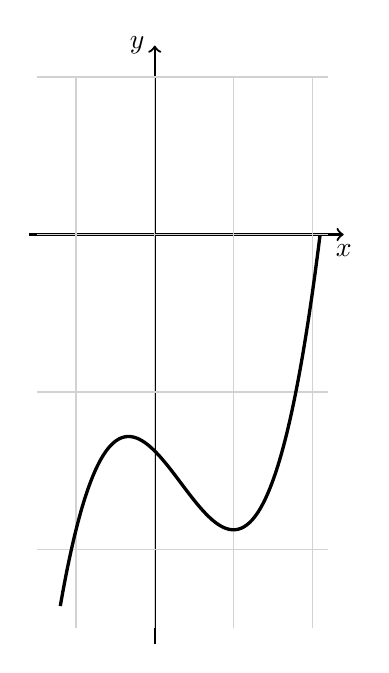
\begin{tikzpicture}[baseline=(current bounding box.center)]
    \draw[->,thick] (-1.6,0) -- (2.4,0) node[below] {$x$};
    \draw[->,thick] (0,-5.2) -- (0,2.4) node[left] {$y$};
    \foreach \y in {-4,-2,0,2} {\draw[gray!35] (-1.5,\y) -- (2.2,\y);}
    \foreach \x in {-1,0,1,2} {\draw[gray!35] (\x,-5) -- (\x,2);}
    \draw[very thick, domain=-1.2:2.1, samples=90, smooth] plot (\x, {\x*\x*\x - \x*\x - \x - 11/4});
  \end{tikzpicture}
\end{center}
\begin{solution}
$-3$
\end{solution}



\newpage



\question[1]
The dynamic pressure $q$ generated by a fluid moving with velocity $v$ is given by
\[
  q = \frac{1}{2} n v^2,
\]
where $n$ is the constant density of the fluid. An aeronautical engineer uses the formula to find the dynamic pressure of a fluid moving with velocity $v$ and with velocity $1.5v$. What is the ratio of the dynamic pressure of the faster fluid to the dynamic pressure of the slower fluid?
\begin{solution}
$2.25$ \quad (\textit{equivalently} $\dfrac{9}{4}$)
\end{solution}

\endgradingrange{sat-drill-00}
